{
\usebackgroundtemplate{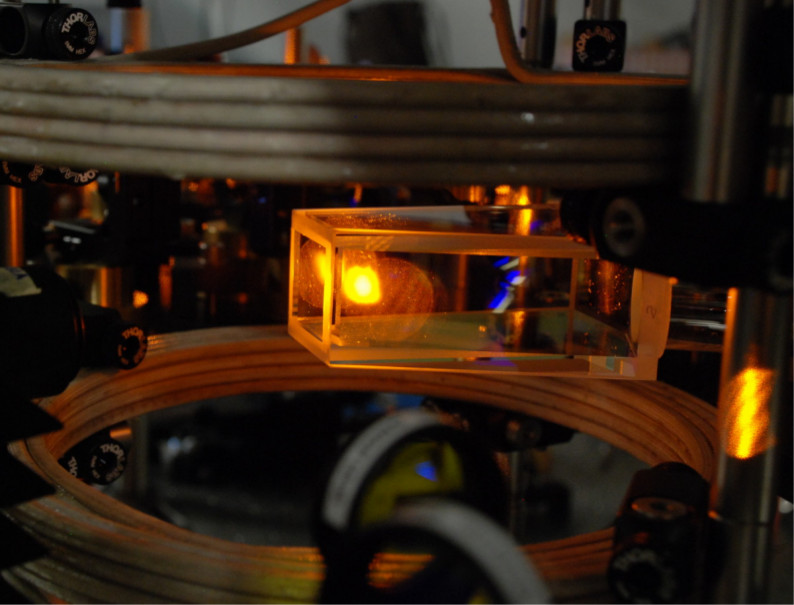
\includegraphics[width=\paperwidth]{Figures/MOT-picture.jpg}}
\begin{frame}<1-3>[t,plain]


\begin{minipage}[c][0.33\textheight][c]{\linewidth}
	\setbeamercolor{title}{fg=white,bg=bellblue}
	\only<1-4>{\pgfsetfillopacity{0.75}}
	\only<5->{\pgfsetfillopacity{0.35}}
	\hfill
	\begin{beamercolorbox}[wd=0.75\linewidth,center,colsep=0.5em,rounded=false]{title}
		\begin{center}
		\only<1-4>{\circled{white}{0.75}{1}\\}
		\only<5->{\circled{white}{0.35}{1}\\} 
		\vspace{1em}
		\textbf{New Bose-Bose mixture} \\
		\vspace{0.5em}
		{\small Miscible, without buoyancy, vicinity to the miscible/immiscible transition}
		\end{center}
	\end{beamercolorbox}
	\hfill\hfill
\end{minipage}

\only<2->{
\begin{minipage}[c][0.33\textheight][c]{\linewidth}
	\setbeamercolor{title}{fg=white,bg=bellblue}
	\only<2,3,5>{\pgfsetfillopacity{0.75}}
	\only<4,6->{\pgfsetfillopacity{0.35}}
	\hfill
	\begin{beamercolorbox}[wd=0.75\linewidth,center,colsep=1em,rounded=false]{title}
		\begin{center}
		\only<2,3,5>{\circled{white}{0.75}{2}\\}
		\only<4,6->{\circled{white}{0.35}{2}\\}
		\vspace{1em}
		\textbf{SD polarizability and oscillation} \\
		\vspace{0.5em}
		{\small Close to the transition: large polarizability, softening of the SD mode.}
		\end{center}
	\end{beamercolorbox}
	\hfill\hfill
\end{minipage}
}

\only<3>{
\begin{minipage}[c][0.33\textheight][c]{\linewidth}
\centering
\textcolor{white}{
\textbf{More info}: 
Arxiv:1607.04574 (2016) \\
\vspace{1em}
\textbf{mail}: tom.bienaime@unitn.it -- \textbf{web}: http://bec.science.unitn.it/
}
\end{minipage}
}
\end{frame}
}
